

%----------------------------------------------------------------------------------------
%   Summary
%----------------------------------------------------------------------------------------



\begin{alertblock}{Summary}
  \begin{wrapfigure}[8]{r}{0.4\textwidth}
    \begin{minipage}{\dimexpr\linewidth-2\fboxrule-2\fboxsep}
    {\tiny
    \begin{lstlisting}
       @ @ @   @       @     @ @     @ @ @     @ @ @ @  @ @ @    @ @ @
      @        @ @   @ @   @     @   @     @   @        @     @  @     @
      @        @   @   @  @       @  @      @  @        @     @  @     @
        @ @    @       @  @       @  @      @  @ @ @    @ @ @    @ @ @
            @  @       @  @       @  @      @  @        @   @    @
            @  @       @   @     @   @     @   @        @    @   @
       @ @ @   @       @     @ @     @ @ @     @ @ @ @  @     @  @

      \  \  /   / /    \   \  /   \  /    /     /        @ @ @   @ @ @
       \ _\/   /_/      \   \/     \/    /_____/        @     @  @     @
           \__/          \  /      _\___/                     @  @      @
               \____      \/      /                          @   @      @
                    \_____/______/                         @     @      @
                                 \                       @       @     @
                                  \____________________ @ @ @ @  @ @ @
    \end{lstlisting}
    }
    \end{minipage}
  \end{wrapfigure}
  In the past parameters of the phy\-sically-based, distributed, event runoff/erosion SMODERP2D Model were inferred for each soil textural class. This approach were performed to simplify practitioners life since the parameters were ready to use if one have the soil texture of the area of interest. In order to assess variability of each parameter within and across textural classes the model were optimized to laboratory artificial rainfall experiments at 4 different textural classes. 
  Results shows that ...
\end{alertblock}\vspace{0.9cm}



%----------------------------------------------------------------------------------------
%   INTRODUCTION
%----------------------------------------------------------------------------------------


\mojesekce{Introduction and Methods}
\subsection{gov}
\begin{block}{Model structure}
    Based on a balance equation 
    $$
        \frac{Storage}{\Delta t} = \nonumber  
        Inflow - Outflow
    $$
    is inferred bucket model with kinematic wave approach for momentum 
    $$
%       \begin{split}
        \frac{\partial h_{i}}{\partial t} =  es_{i} + \sum_j^n q_{j} - inf_{i} - q_{i} - ret_i
    $$
    where $h$ is water level [$L$], $es$ is effective precipitation [$L.T^{-1}$], $inf$ is infiltration [$L.T^{-1}$], $ret$ surface retention [$L$], and $q$ is the Manning-Strickler formula
    $$
      q = Xi^Yh^b. 
    $$
    Parameters $X$, $Y$, and $b$ were inferred for each soil textural class. Variability of those parameters within and among textural classes is assessed in this poster. 
\end{block}





\subsection{Soil classes and ARE overview}
\begin{block}{Soil classes and ARE overview}

\begin{columns}
    \begin{column}{0.4\textwidth}
        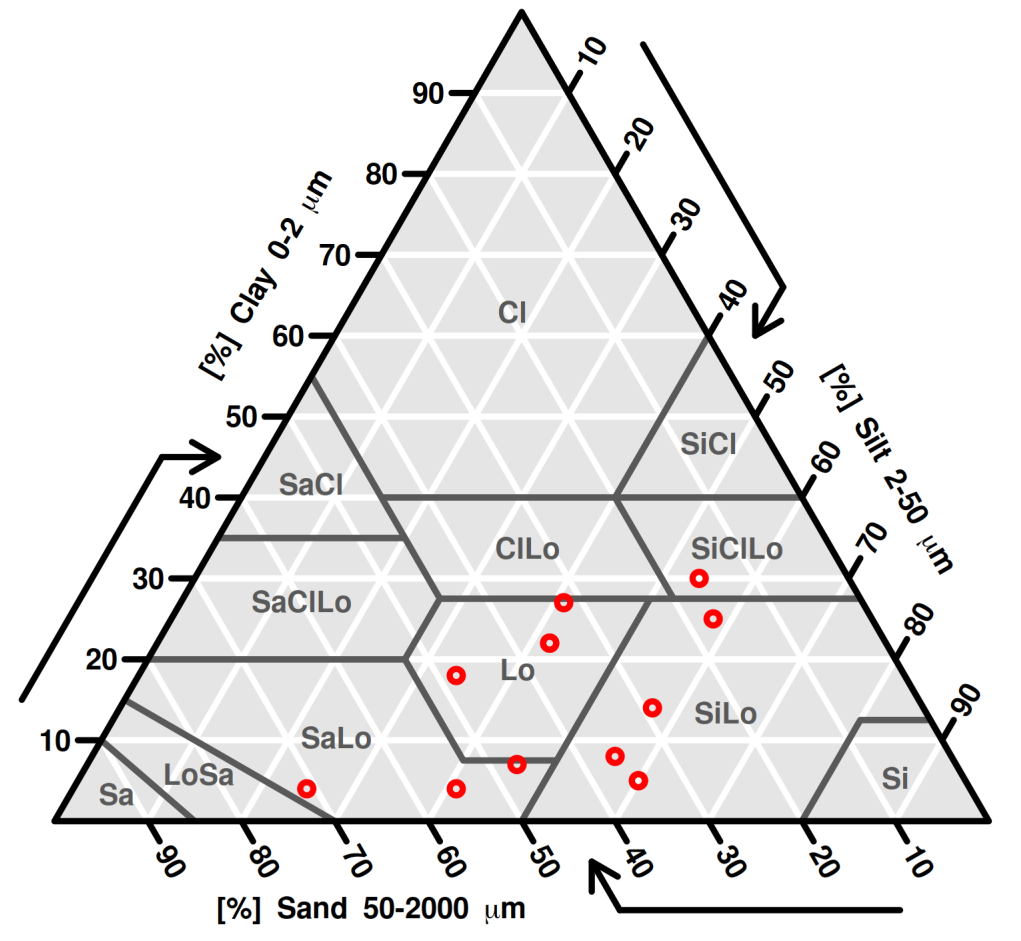
\includegraphics[width=1.1\textwidth]{obr/soil_triangle.png}
    \end{column}
    \begin{column}{0.6\textwidth}
        \begin{table}[]
        \begin{tabular}{lcccccc}
        \hline
        \hline
        location      & year    & no. of            & \multicolumn{3}{c}{soil texture {[}\%{]}}  & soil class      \\
                    &         & exper.       & clay  & silt  & sand &  \\
        \hline
        Horoměřice    & 2002    & 25                & 25             & 58            & 17            & silty loam      \\
        Třebsín I     & 2004    & 22                & 5              & 60            & 35            & silty loam      \\
        Neustupov     & 2006    & 14                & 4              & 41            & 55            & sandy loam      \\
        Klapý         & 2007    & 25                & 30             & 54            & 16            & silty clay loam \\
        Třebsín II    & 2008    & 28                & 5              & 60            & 35            & silty loam      \\
        Třebešice I   & 2009    & 27                & 4              & 25            & 71            & sandy loam      \\
        Třebešice II  & 2010    & 36                & 7              & 46            & 47            & sandy loam      \\
        Nučice        & 2011    & 35                & 14             & 57            & 29            & silty loam      \\
        Všetaty I     & 2012    & 24                & 22             & 42            & 36            & loam            \\
        Všetaty II    & 2013    & 17                & 22             & 42            & 36            & loam            \\
        Třebešice III & 2014    & 22                & 8              & 56            & 36            & silty loam      \\
        Nové Strašecí & 2015    & 20                & 27             & 41            & 32            & loam            \\
        Řisuty        & 2017    & 21                & 18             & 34            & 48            & loam           \\
        \hline
        \hline
        \end{tabular}
        \end{table}
    \end{column}
\end{columns}


\end{block}


\subsection{Modeling exercises}
\begin{block}{Modeling exercises}
Sensitivity analyses\\
Model optimization\\
Uncertainty analyses - monte carlo


\end{block}
% \end{block}








        
